\documentclass[12pt,a4paper]{article}

\usepackage{listings}
\usepackage{xcolor}
\usepackage{amsmath}
\usepackage{graphicx}
\usepackage{tikz}
\usetikzlibrary{arrows.meta}

% location of the images directory
\graphicspath{ {./Graphs/} }


% define custom colors and style for the code section
\definecolor{backcolor}{rgb}{0.95,0.95,0.95}
\definecolor{commentcolor}{rgb}{0.5,0.5,0.5}

\lstdefinestyle{mystyle}{
    backgroundcolor=\color{backcolor},
    basicstyle=\ttfamily\footnotesize,
    commentstyle=\color{commentcolor},
    breakatwhitespace=false,   
    showstringspaces=false,
    numbers=left,
    frame=shadowbox,
    breaklines=true,
    captionpos=b
}

\lstset{style=mystyle}

% preamble
\title{ 
	Sistema MM1 \\
	\large Simulazione di un sistema a coda }
\author{Pietro Casavecchia}
\date{\today}


\begin{document}
\maketitle

\vspace*{\stretch{1}}
\begin{center}
\scalebox{0.75}{
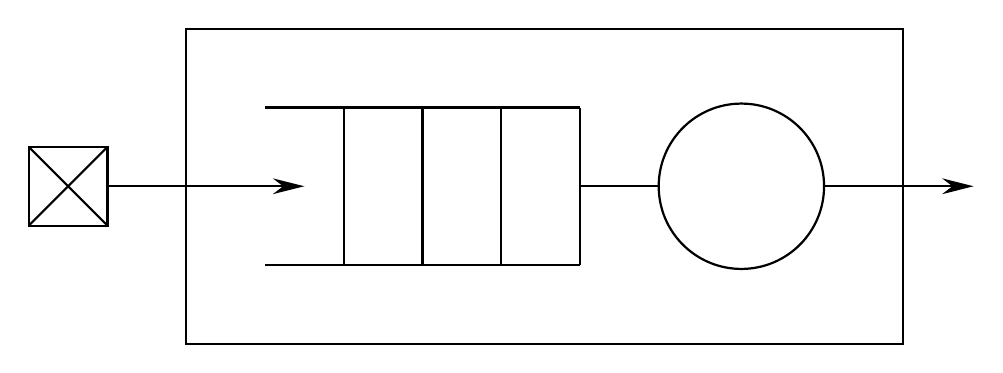
\begin{tikzpicture}
\draw [thick] (0,4) rectangle (1,5);
\draw [thick] (0,4) -- (1,5);
\draw [thick] (1,4) -- (0,5);
\draw [thick] [-{Stealth[length=4mm, width=2mm]}] (1,4.5) -> (3.5,4.5);
\draw [thick] (2,2.5) rectangle (11.1,6.5);
\draw [thick] (3,3.5) -- (7,3.5);
\draw [thick] (3,5.5) -- (7,5.5);
\draw [thick] (4,3.5) -- (4,5.5);
\draw [thick] (5,3.5) -- (5,5.5);
\draw [thick] (6,3.5) -- (6,5.5);
\draw [thick] (7,3.5) -- (7,5.5);
\draw [thick] (7,4.5) -- (8,4.5);
\draw [thick] (9.05,4.5) circle (10.5mm);
\draw [thick] [-{Stealth[length=4mm, width=2mm]}] (10.1,4.5) -> (12,4.5);
\end{tikzpicture}
}
\end{center}
\vspace*{\stretch{1}}

\thispagestyle{empty}
\newpage

\tableofcontents

\newpage

\raggedright
\noindent
\section{Obbiettivo}
L'obbiettivo è quello di simulare il sistema a coda MM1. \\
Si è cercato di rimanere fedeli al reale funzionamento cercando di interpretare il significato fisico delle componenti del sistema e implementare i funzionamenti in modo da potere essere vicini ad una rappresentazione reale.

\section{Struttura}
Il progrmma è stutturato in classi corrispondenti agli oggetti del sistema che sono:
\begin{itemize}
  \item Class Package
  \item Class Buffer
  \item Class Server
  \item Class System
\end{itemize}

\subsection{Funzione delle Classi}
L'obbiettivo delle Classi Package, Buffer e Server è quello di creare, nel caso del pacchetto più istanze quindi più oggetti definiti come pacchetti mentre le altre due Classi sono chiamate solo una volta così da creare un oggetto che rappresenti una Buffer e un Server.
\bigbreak
La Classe System rappresenta l'intero sistema, gestisce le altre classi e nel caso del Buffer e del Server li chiama una volta sola, mentre chiama la Classe Package ogni volta che un nuovo pacchetto si deve generare. \\
Inoltre System genera i pacchetti, siccome un Metodo di generazione nella Classe Package non avrebbe senso perchè sarebbe legato a tutti i pacchetti, mentre è necessario avere un Metodo di generazione che comprenda tutti i Pacchetti quindi deve essere un Metodo della Classe System.
\subsection{Tempo nella Simulazione}
Il tempo è rappresentato da UT quindi Unità di Tempo indefinita, ogni UT è un ciclo di un While che dura fino al tempo di osservazione del sistema. \\
Per ogni UT vengono chiamate tutte funzioni principali.

\section{Codice}
Il codice è diviso in Classi e Funzioni per statistiche e plot del Sistema.

\subsection{Class Package}
\begin{lstlisting}[language=Python, caption=Class Package]
class Package:
    def __init__(self):
        self.id_number = None
\end{lstlisting}

\subsection{Class Buffer}
\begin{lstlisting}[language=Python, caption=Class Buffer]
class Buffer:
    def __init__(self):
        self.queue = []
    
    def calculate_buffer_size(self):
        return len(self.queue)
\end{lstlisting}

\subsection{Class Server init}
\begin{lstlisting}[language=Python, caption=Class Server init]
class Server:
    def __init__(self):
        self.pkg_serving = None
        self.status = 0
        self.serving_time = None
        self.service_progression = None

        # parameters and feedback
        self.array_serving_time = []
\end{lstlisting}

\newpage
\subsection{Server Methods}
\begin{lstlisting}[language=Python, caption=Server Methods]
def from_buffer_to_server(self, buffer):
    # FIFO buffer
    # get first pkg
    pkg = buffer.queue[0]
    # eliminate from queue
    buffer.queue.pop(0)
    # move into the server change server status
    self.status = 1
    self.pkg_serving = pkg

    # generate a serving time > 0
    while True:
        self.serving_time = math.floor(np.random.exponential(S))
        if self.serving_time > 0:
            break
    # initiate service progression 
    self.service_progression = 0

    # append serving time for feedback 
    self.array_serving_time.append(self.serving_time)

def service(self, buffer, pkgs_served):
    # if status of the server is zero and a pkg in 
    # 	the buffer exits then move the pkg 
    # 	into the server
    if self.status == 0 and buffer.calculate_buffer_size() == 0:
        # erase pkg given exited the server 
        self.pkg_serving = None
        # empty the server 
        self.serving_time = None
        self.service_progression = None
    elif self.status == 0 and buffer.calculate_buffer_size() > 0:
        self.from_buffer_to_server(buffer)

    # if the serving time == 0 then after the 
    # 	from_buffer...() call the status will be 1 
    if self.status == 1:
        self.service_progression += 1
        if self.service_progression > self.serving_time:
            # append in pkgs served
            pkgs_served.append(self.pkg_serving)
            self.status = 0
\end{lstlisting}


\subsection{Class System init}
\begin{lstlisting}[language=Python, caption=Class System init]
class System():
    def __init__(self, run_time, IA):
        self.IA = IA
        self.run_time = run_time
        self.current_time = 0
        self.n_pkgs = 0
        self.pkgs_served = []

        # generation of pkg variabiles
        self.inter_arrival_time = None
        self.generation_progression = None

        # generate a buffer and server
        self.buffer = Buffer()
        self.server = Server()

        # parameters and feedback
        # number of pkgs nel sistema for every unit of time 
        self.array_inter_arrival_time = []
        self.pkgs_sys_for_unitTime = []
        self.pkgs_queue_for_unitTime = []
        self.dict_pkgsTime_queue = {}
        self.dict_pkgsTime_system = {}
        # array counter for how many pkgs in the 
        # 	system [a, b]
        # a: how many time there are none and b: 
        # 	how many time there > 0
        self.array_P01 = [0, 0]

        # start simulation call
        self.simulation()
\end{lstlisting}

\subsection{System Method Pkg Generation}
\begin{lstlisting}[language=Python, caption=System Method Pkg Generation]
def pkg_generation(self):
    # initialize pkg to none 
    pkg = None
    # run the generation only for the run time time 
    if self.current_time < self.run_time:
        # generate pkg zero
        if (
            (self.current_time == 0) or 
            (self.generation_progression >= self.inter_arrival_time)
            ):
            pkg = Package()
            pkg.id_number = self.n_pkgs
            self.n_pkgs += 1
            # inter arrival time > 0
            while True:
                self.inter_arrival_time = math.floor(np.random.exponential(self.IA))
                if self.inter_arrival_time > 0:
                    break
            # set generation progression to zero for initialize it 
            self.generation_progression = 0

            # append gen time for feedback 
            self.array_inter_arrival_time.append(self.inter_arrival_time)
        
        # increment only if self.inter_arrival_time != 0 
        # because the pkg gen fn will be called again
        if self.inter_arrival_time != 0:
            self.generation_progression += 1
    else: 
        self.inter_arrival_time = None
        self.generation_progression = None
    
    return pkg 
\end{lstlisting}


\subsection{System Method Simulation}
\begin{lstlisting}[language=Python, caption=System Method Simulation]
def simulation(self): 
    # do not continue the process until all pks are served 
    # 	end with run time 
    while (self.current_time < self.run_time):

        # --- --- --- start sys call --- --- --- 

        # menage generation 
        pkg = self.pkg_generation()
        # manage buffer 
        if pkg != None: self.buffer.queue.append(pkg)
        # manage server
        self.server.service(self.buffer, self.pkgs_served)

        # --- --- --- end sys call --- --- ---
         
		# --- --- --- start print df --- --- ---
        # print pkg
        if pkg == None: data_list.append(None)
        elif pkg != None: data_list.append(pkg.id_number)

        # print buffer
        queue_pkgs = []
        for i in range(len(self.buffer.queue)):
            queue_pkgs.append(self.buffer.queue[len(self.buffer.queue) - i - 1].id_number)
        data_list.append(queue_pkgs)
        data_list.append(self.buffer.calculate_buffer_size())

        # print server 
        printServerStatus = "-->" if self.server.status == 1 else "None"
        data_list.append(printServerStatus)

        # print pkg served 
        if self.server.pkg_serving == None: data_list.append(None)
        elif self.server.pkg_serving != None: data_list.append(self.server.pkg_serving.id_number)
        data_list.append(self.server.serving_time)
        data_list.append(self.server.service_progression)
        
        # print sys
        last_served_pkgs = []
        for i in range(len(self.pkgs_served)):
            if i >= 5: break
            last_served_pkgs.append(self.pkgs_served[len(self.pkgs_served) - i - 1].id_number)
        data_list.append(len(self.pkgs_served))
        data_list.append(last_served_pkgs)

        # append to the last index of df that is the len(df)
        df.loc[len(df)] = data_list
        # --- --- --- end print df --- --- ---

        # --- --- --- start feedback --- --- ---
        # Ls Lq
        self.pkgs_sys_for_unitTime.append(self.n_pkgs - len(self.pkgs_served))
        self.pkgs_queue_for_unitTime.append(self.n_pkgs - len(self.pkgs_served) - self.server.status)
        # calculate how long a pkg in the queue
        for i in range(len(self.buffer.queue)):
            # get value of  pkg 
            value_queue_pkg = self.dict_pkgsTime_queue.get(self.buffer.queue[i].id_number)
            # if is none set to 1 else increment by 1 
            if value_queue_pkg == None:
                self.dict_pkgsTime_queue.update({self.buffer.queue[i].id_number: 1})
            else:
                self.dict_pkgsTime_queue.update({self.buffer.queue[i].id_number: value_queue_pkg + 1})
        # calculate how long a pkg in the server 
        # read the value in the server 
        #   check if already exits in the dict then 
        # 		add 1 else increase by one 
        if self.server.pkg_serving != None:
            # search it in the 
            value_server_pkg = self.dict_pkgsTime_system.get(self.server.pkg_serving.id_number)
            if value_server_pkg == None:
                self.dict_pkgsTime_system.update({self.server.pkg_serving.id_number: 1})
            else:
                self.dict_pkgsTime_system.update({self.server.pkg_serving.id_number: value_server_pkg + 1})
        # calculate value probability 0 add it to array 
        # 	first index is when queue
        if len(self.buffer.queue) == 0 and self.server.status == 0:
            self.array_P01[0] += 1
        else:
            self.array_P01[1] += 1
        # --- --- --- end feedback --- --- ---
        
        print(self.n_pkgs, end="\r")

        # increment simulation time 
        self.current_time += 1
\end{lstlisting}

\newpage
\subsection{System Method Parameters}
\begin{lstlisting}[language=Python, caption=System Method Parameters]
def calculate_parameters(self):
    # take the value from the dict of waiting 
    # 	time in the server / queue
    array_waitingTime_queue = []
    array_waitingTime_server = []
    for values_q in self.dict_pkgsTime_queue.values():
        array_waitingTime_queue.append(values_q)
    # adjust with adding 1 for mean for missing pks 
    for _ in range(self.n_pkgs - len(array_waitingTime_queue)):
        array_waitingTime_queue.append(0)

    for values_s in self.dict_pkgsTime_system.values():
        array_waitingTime_server.append(values_s)
    # adjust with adding 1 for mean for missing pks 
    for _ in range(self.n_pkgs - len(array_waitingTime_server)):
        array_waitingTime_server.append(0)


    return (
        self.array_inter_arrival_time,
        self.server.array_serving_time,
        self.pkgs_sys_for_unitTime,  
        self.pkgs_queue_for_unitTime,
        array_waitingTime_server,
        array_waitingTime_queue,
        self.array_P01
        )
\end{lstlisting}

\newpage
\section{Sezione della Simulazione}
\begin{lstlisting}[language=bash, caption=System Section]
    UT interTime genProc pkgIdGen      queue  buffDim  \
0    0      None    None        0         []        0   
1    1         1       1        1        [1]        1   
2    2         1       1        2        [2]        1   
3    3         3       1     None        [2]        1   
4    4         3       2     None        [2]        1   
5    5         3       3        3     [3, 2]        2   
6    6         1       1        4     [4, 3]        2   
7    7         1       1        5     [5, 4]        2   
8    8         2       1     None     [5, 4]        2   
9    9         2       2        6  [6, 5, 4]        3   
10  10         3       1     None     [6, 5]        2   
11  11         3       2     None     [6, 5]        2   
12  12         3       3        7  [7, 6, 5]        3   
13  13         5       1     None     [7, 6]        2   
14  14         5       2     None     [7, 6]        2   

   servStatus  pkgIdServ  servTime  servProc  nPkgsServ  \
0         -->          0         2         1          0   
1        None          0         2         2          1   
2         -->          1         4         1          1   
3         -->          1         4         2          1   
4         -->          1         4         3          1   
5        None          1         4         4          2   
6        None          2         1         1          3   
7         -->          3         3         1          3   
8         -->          3         3         2          3   
9        None          3         3         3          4   
10        -->          4         3         1          4   
11        -->          4         3         2          4   
12       None          4         3         3          5   
13        -->          5         4         1          5   
14        -->          5         4         2          5   

         pkgsServed  
0                []  
1               [0]  
2               [0]  
3               [0]  
4               [0]  
5            [1, 0]  
6         [2, 1, 0]  
7         [2, 1, 0]  
8         [2, 1, 0]  
9      [3, 2, 1, 0]  
10     [3, 2, 1, 0]  
11     [3, 2, 1, 0]  
12  [4, 3, 2, 1, 0]  
13  [4, 3, 2, 1, 0]  
14  [4, 3, 2, 1, 0]  
\end{lstlisting}


\subsection{Grafici Pkgs nel Sistema per Unità di Tempo}
Il primo rappresenta la sezione fino a 15ut, invece il secondo una simulazione con lo stesso Seed fino a 500ut

\begin{figure}[h]
\centering
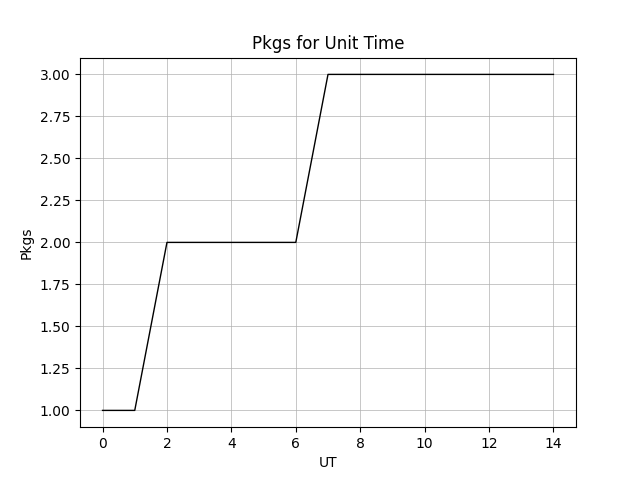
\includegraphics[scale=0.6]{PkgsUT}
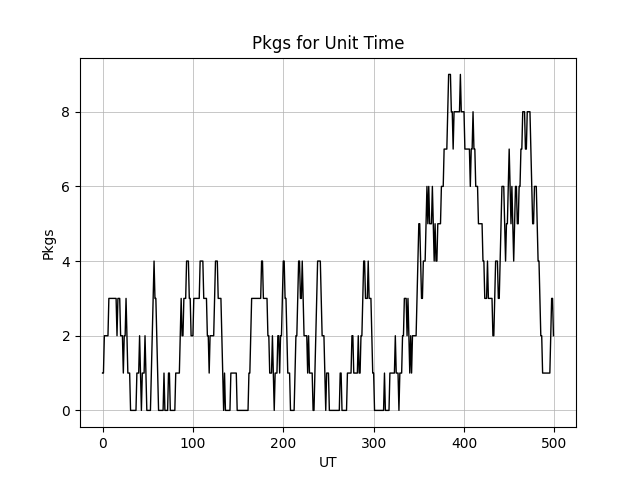
\includegraphics[scale=0.6]{PkgsUT_Long}
\end{figure}

\newpage
\section{Parametri del Sistema}
Vengono calcolati i parametri teorici usando le seguenti equazioni, poi vengono calcolati i parametri sperimentali, concretizzando il significato pratico delle equazioni mettendo degli appositi Flag nella simulazione, cosi da avere per ogni parametro teorico il corrispettivo sperimentale. \\
Viene calcolato anche $\lambda$ e $\mu$ sperimentale osservando il Tempo di Interarrivo (IA) e il Tempo di Servizio (S) generati dalle opportune distribuzioni esponenziali. 

\subsection{Equazioni}
Dato il Tempo di Interarrivo: IA e il Tempo di Servizio S:
\begin{align*}
\lambda  &= \frac{1}{IA} & 
\mu &= \frac{1}{S}
\end{align*}

Steady State:
\begin{align*}
\lambda_k &= \lambda & 
\mu_k &= \mu
\end{align*}

Fattore di utilizzo o percentuale del tempo che tutti i Servers sono accupati: 
\begin{align*}
\rho &= \frac{\lambda}{\mu} & 
\rho &= 1 - P_0
\end{align*}

$P_0$ Probabilità di avere $0$ Pkgs nel Sistema:
\begin{align*}
P_0 = 1 - \frac{\lambda}{\mu} = 1 - \rho
\end{align*}

$P_k$ Probabilità di avere $k$ Pkgs nel Sistema:
\begin{align*}
P_k = P_0 \bigg(\frac{\lambda}{\mu}\bigg)^k = \rho^k \cdot P_0
\end{align*}

$W_S$ Tempo medio di un Pkg nel Sistema, $W_q$ tempo medio di un Pkg nel Buffer:
\begin{align*}
W_S &= \frac{L_S}{\lambda} = \frac{1}{\mu - \lambda} &
W_q &= W_S - \frac{1}{\mu} = \frac{\lambda}{\mu(\mu - \lambda)}
\end{align*}

$L_S$ Numero medio di Pkgs nel Sistema, $L_q$ Numero medio di Pkgs nel Buffer:
\begin{align*}
L_S &= \frac{\rho}{1 - \rho} &
L_q &= \frac{\lambda^2}{\mu(\mu - \lambda)} = \lambda W_q = \frac{\rho^2}{1 - \rho}
\end{align*}


\subsection{Esempio Output con $\lambda$ e $\mu$ Fissati}
Viene fissato il Tempo di Interarrivo e il Tempo di Servizio quindi di conseguenza $\lambda$ e 
$\mu$ poi vengono fatte $n$ simulazione per avere un valore medio dei parametri, in questo caso il numero di simulazioni era 5 con un Tempo di Simulazione di 40000ut. 
\bigbreak
\begin{lstlisting}[language=bash, caption=Output Parameters Sample]
IA theo: 18.5 IA out: 21.816 error: 17
S theo: 5 S out: 5.532 error: 10
Lambda theo: 0.054 Lambda out: 0.046 error: -15
Mu theo: 0.2 Mu out: 0.181 error: -10
Rho theo: 0.27 Rho out: 0.256 error: -6
Ls theo: 0.37 Ls out: 0.35 error: -6
Lq theo: 0.1 Lq out: 0.094 error: -7
Ws theo: 6.852 Ws out: 8.546 error: 24
Wq theo: 1.852 Wq out: 2.015 error: 8
P0 theo: 0.73 P0 out: 0.732 error: 0
\end{lstlisting}

\subsection{Parametro P}
Grafico teorico e sperimentale dell'andamento di $Pk$ in funzione di $k$ tenendo $\rho$ costante, il massimo $k$ in questo caso si è scelto arbitrariamente per semplicià ma si potrebbe scegliere il massimo $k$ osservato nella simulazione.
\begin{figure}[h]
\centering
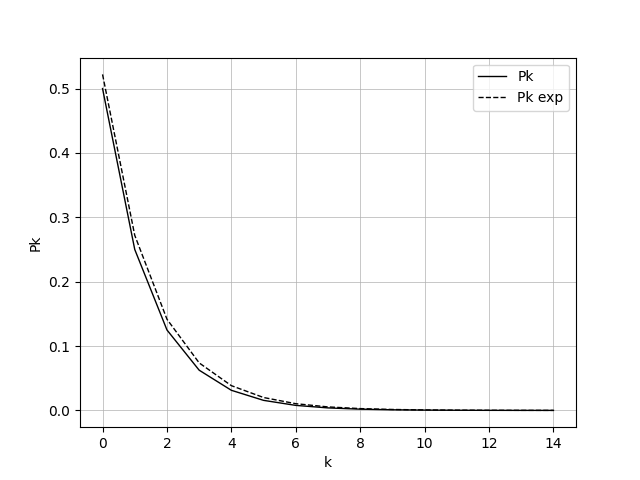
\includegraphics[scale=0.6]{Pk}
\end{figure}

\newpage
\subsection{Output con Variazione di $\rho$}
Si è fissato il Tempo di Servizio e si è fatto variare in modo incrementale il Tempo di Interarrivo mantenendo sempre valida la relazione:


\begin{align*}
\lambda &< \mu & (IA) &> S & 0 < \rho < 1
\end{align*}

\subsection{Parametro W}
Grafico teorico e sperimentale dell'andamento di $W_S$ e $W_q$ in funzione di $\rho$
\begin{figure}[h]
\centering
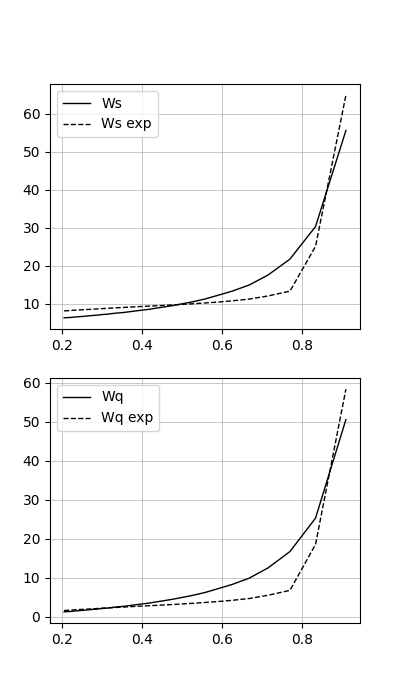
\includegraphics[scale=0.8]{W}
\end{figure}

\subsection{Parametro L}
Grafico teorico e sperimentale dell'andamento di $L_S$ e $L_q$ in funzione di $\rho$
\begin{figure}[h]
\centering
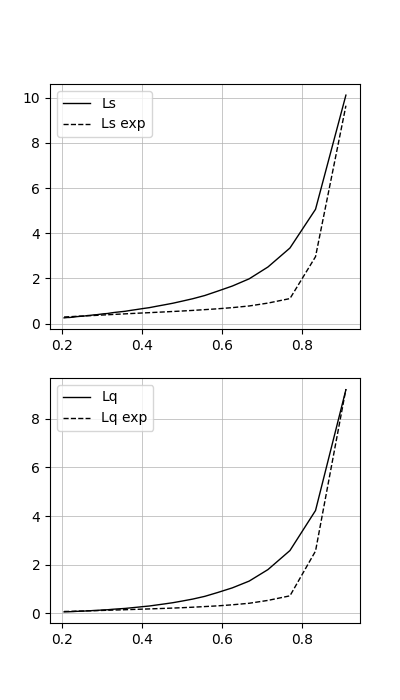
\includegraphics[scale=0.8]{L}
\end{figure}


\newpage
\section{Considerazioni}
Di seguito vengono elencate le principali considerazioni fatte per la simulazione.
\subsection{Scarto dello Zero}
Usando appropriate distribuzioni esponenziali per la generazione di $\lambda$ e $\mu$, vengono eliminati i casi nei quali restituiscono valore $0$ perchè essendo la simulazione in tempi discreti si avrebbero multipli arrivi e servizi nella stessa Unità di Tempo, anche se potrebbe essere una buona approssimazione della realtà, si intende un UT molto piccola che quindi non permette piu di un arrivo o servizio.
\subsection{Osservazione della Simulazione}
Il tempo di osservazione della simulazione parte da un tempo $t=0$ e finisce in un tempo $t=end$ quindi non si ferma la generazione dei Pkgs e poi si aspetta il loro servizio ma si smette di osservare il sistema quando ancora i Pkgs si stanno generando.
Più $\rho$ è piccolo più la differenza tra questi due approcci è meno significativa perchè c'è meno utilizzo dei Server e quindi meno Pkgs da servire dopo la fine della generazione.
\subsection{Lungezza della Simulazione}
Più la simulazione è lunga in UT più si da spazio a tempi di generazione e servizio più lunghi.
\subsection{Errore in funzione di Rho}
Più $\rho$ è grande più l'errore su i parametri aumenta.


\newpage
\lstlistoflistings

\end{document}